%!TEX TS-program = xelatex
%!TEX encoding = UTF-8 Unicode
% Awesome CV LaTeX Template for CV/Resume
%
% This template has been downloaded from:
% https://github.com/posquit0/Awesome-CV
%
% Author:
% Claud D. Park <posquit0.bj@gmail.com>
% http://www.posquit0.com
%
%
% Adapted to be an Rmarkdown template by Mitchell O'Hara-Wild
% 23 November 2018
%
% Template license:
% CC BY-SA 4.0 (https://creativecommons.org/licenses/by-sa/4.0/)
%
%-------------------------------------------------------------------------------
% CONFIGURATIONS
%-------------------------------------------------------------------------------
% A4 paper size by default, use 'letterpaper' for US letter
\documentclass[11pt, a4paper]{awesome-cv}

% Configure page margins with geometry
\geometry{left=1.4cm, top=.8cm, right=1.4cm, bottom=1.8cm, footskip=.5cm}

% Specify the location of the included fonts
\fontdir[fonts/]

% Color for highlights
% Awesome Colors: awesome-emerald, awesome-skyblue, awesome-red, awesome-pink, awesome-orange
%                 awesome-nephritis, awesome-concrete, awesome-darknight

\definecolor{awesome}{HTML}{009ACD}

% Colors for text
% Uncomment if you would like to specify your own color
% \definecolor{darktext}{HTML}{414141}
% \definecolor{text}{HTML}{333333}
% \definecolor{graytext}{HTML}{5D5D5D}
% \definecolor{lighttext}{HTML}{999999}

% Set false if you don't want to highlight section with awesome color
\setbool{acvSectionColorHighlight}{true}

% If you would like to change the social information separator from a pipe (|) to something else
\renewcommand{\acvHeaderSocialSep}{\quad\textbar\quad}

\def\endfirstpage{\newpage}

%-------------------------------------------------------------------------------
%	PERSONAL INFORMATION
%	Comment any of the lines below if they are not required
%-------------------------------------------------------------------------------
% Available options: circle|rectangle,edge/noedge,left/right

\photo{photo.jpg}
\name{Lampros Sp. Mouselimis}{}


\email{\href{mailto:mouselimislampros@gmail.com}{\nolinkurl{mouselimislampros@gmail.com}}}
\homepage{mlampros.github.io/}
\orcid{0000-0002-8024-1546}
\googlescholar{JXg3b58AAAAJ}
\github{mlampros}
\linkedin{mlampros}
\twitter{lampros\_twit}

% \gitlab{gitlab-id}
% \stackoverflow{SO-id}{SO-name}
% \skype{skype-id}
% \reddit{reddit-id}

\quote{I'm a data \& remote sensing analyst and open source author /
maintainer of numerous R language packages (CRAN, Github), competent in
two programming languages (R, Python) who takes advantage of C++ (in R
through the Rcpp and RcppArmadillo packages and in python through
Cython) to improve the efficiency of internal functions}

\usepackage{booktabs}

\providecommand{\tightlist}{%
	\setlength{\itemsep}{0pt}\setlength{\parskip}{0pt}}

%------------------------------------------------------------------------------


\usepackage{float}
\floatplacement{figure}{H}

% Pandoc CSL macros
\newlength{\cslhangindent}
\setlength{\cslhangindent}{1.5em}
\newlength{\csllabelwidth}
\setlength{\csllabelwidth}{3em}
\newenvironment{CSLReferences}[3] % #1 hanging-ident, #2 entry spacing
 {% don't indent paragraphs
  \setlength{\parindent}{0pt}
  % turn on hanging indent if param 1 is 1
  \ifodd #1 \everypar{\setlength{\hangindent}{\cslhangindent}}\ignorespaces\fi
  % set entry spacing
  \ifnum #2 > 0
  \setlength{\parskip}{#2\baselineskip}
  \fi
 }%
 {}
\usepackage{calc}
\newcommand{\CSLBlock}[1]{#1\hfill\break}
\newcommand{\CSLLeftMargin}[1]{\parbox[t]{\csllabelwidth}{#1}}
\newcommand{\CSLRightInline}[1]{\parbox[t]{\linewidth - \csllabelwidth}{#1}}
\newcommand{\CSLIndent}[1]{\hspace{\cslhangindent}#1}

\begin{document}

% Print the header with above personal informations
% Give optional argument to change alignment(C: center, L: left, R: right)
\makecvheader

% Print the footer with 3 arguments(<left>, <center>, <right>)
% Leave any of these blank if they are not needed
% 2019-02-14 Chris Umphlett - add flexibility to the document name in footer, rather than have it be static Curriculum Vitae
\makecvfooter
  {February 2024}
    {Lampros Sp. Mouselimis~~~·~~~Curriculum Vitae}
  {\thepage}


%-------------------------------------------------------------------------------
%	CV/RESUME CONTENT
%	Each section is imported separately, open each file in turn to modify content
%------------------------------------------------------------------------------



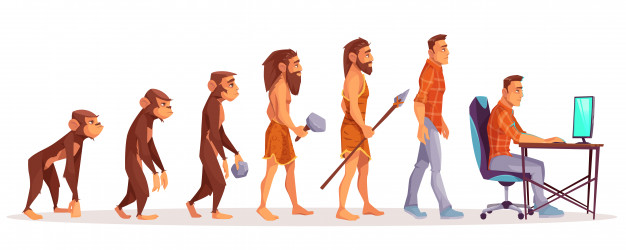
\includegraphics{human_evolution.jpg}

\hypertarget{r-programming-packages}{%
\section{R-Programming Packages}\label{r-programming-packages}}

\begin{cventries}
    \cventry{GLCM Texture Features}{fastGLCM}{Author and maintainer (CRAN)}{2022-08-15}{\begin{cvitems}
\item http://mlampros.github.io/2022/08/16/gray\_level\_co\_occurrence\_matrix/
\end{cvitems}}
    \cventry{Variational Mode Decomposition}{VMDecomp}{Author and maintainer (CRAN)}{2022-06-09}{\begin{cvitems}
\item http://mlampros.github.io/2022/06/11/variatonal\_mode\_decomposition/
\end{cvitems}}
    \cventry{ICESat-2 Altimeter Data using R}{IceSat2R}{Author and maintainer (CRAN)}{2022-02-07}{\begin{cvitems}
\item http://mlampros.github.io/2022/02/12/IceSat2R\_Altimetry\_data/
\end{cvitems}}
    \cventry{Processing of the 'Planet NICFI' Satellite Imagery}{PlanetNICFI}{Author and maintainer (CRAN)}{2021-06-10}{\begin{cvitems}
\item http://mlampros.github.io/2021/06/12/Planet\_NICFI\_Satellite\_Imagery/
\end{cvitems}}
    \cventry{`Fitbit' Visualizations}{fitbitViz}{Author and maintainer (CRAN)}{2021-05-18}{\begin{cvitems}
\item http://mlampros.github.io/2021/05/20/fitbitViz\_package/
\end{cvitems}}
    \cventry{Copernicus Digital Elevation Models}{CopernicusDEM}{Author and maintainer (CRAN)}{2021-05-15}{\begin{cvitems}
\item http://mlampros.github.io/2021/05/21/copernicusDEM\_package/
\end{cvitems}}
    \cventry{Efficient Learning of Word Representations and Sentence Classification}{fastText}{Author and maintainer (CRAN)}{2021-05-14}{\begin{cvitems}
\item http://mlampros.github.io/2021/05/14/fasttext\_language\_identification/
\end{cvitems}}
    \cventry{Superpixel Image Segmentation}{SuperpixelImageSegmentation}{Author and maintainer (CRAN)}{2018-12-30}{\begin{cvitems}
\item http://mlampros.github.io/2018/11/09/Image\_Segmentation\_Superpixels\_Clustering/
\end{cvitems}}
    \cventry{The Extreme Learning Machine Algorithm}{elmNNRcpp}{Author and maintainer (CRAN)}{2018-07-05}{\begin{cvitems}
\item http://mlampros.github.io/2018/07/05/the\_extreme\_learning\_machine\_package/
\end{cvitems}}
    \cventry{Non Metric Space (Approximate) Library}{nmslibR}{Author and maintainer (CRAN)}{2018-02-27}{\begin{cvitems}
\item http://mlampros.github.io/2018/02/27/the\_nmslibR\_package/
\end{cvitems}}
    \cventry{Regularized Greedy Forest}{RGF}{Author and maintainer (CRAN)}{2018-02-13}{\begin{cvitems}
\item http://mlampros.github.io/2018/02/14/the\_RGF\_package/
\end{cvitems}}
    \cventry{Geospatial Queries Using `PyMongo'}{GeoMongo}{Author and maintainer (CRAN)}{2017-08-07}{\begin{cvitems}
\item http://mlampros.github.io/2017/08/07/the\_GeoMongo\_package/
\end{cvitems}}
    \cventry{Fuzzy String Matching}{fuzzywuzzyR}{Author and maintainer (CRAN)}{2017-04-11}{\begin{cvitems}
\item http://mlampros.github.io/2017/04/13/fuzzywuzzyR\_package/
\end{cvitems}}
    \cventry{A GeoJson Processing Toolkit}{geojsonR}{Author and maintainer (CRAN)}{2017-03-28}{\begin{cvitems}
\item http://mlampros.github.io/2017/03/29/geojsonR\_package/
\end{cvitems}}
    \cventry{Text Processing for Small or Big Data Files}{textTinyR}{Author and maintainer (CRAN)}{2017-01-07}{\begin{cvitems}
\item http://mlampros.github.io/2017/01/05/textTinyR\_package/
\end{cvitems}}
    \cventry{Global Vectors for Word Representation (Glove)}{GloveR}{Author and maintainer (Github)}{2017-01-04}{\begin{cvitems}
\item https://mlampros.github.io/GloveR/
\end{cvitems}}
    \cventry{Random Search in R}{RandomSearchR}{Author and maintainer (Github)}{2016-09-19}{\begin{cvitems}
\item http://mlampros.github.io/2016/03/14/random\_search\_R/
\end{cvitems}}
    \cventry{Gaussian Mixture Models, K-Means, Mini-Batch-Kmeans, K-Medoids and Affinity Propagation Clustering}{ClusterR}{Author and maintainer (CRAN)}{2016-09-06}{\begin{cvitems}
\item http://mlampros.github.io/2016/09/12/clusterR\_package/
\end{cvitems}}
    \cventry{Kernel k Nearest Neighbors}{KernelKnn}{Author and maintainer (CRAN)}{2016-07-11}{\begin{cvitems}
\item http://mlampros.github.io/2016/07/10/KernelKnn/
\end{cvitems}}
    \cventry{An Image Processing Toolkit}{OpenImageR}{Author and maintainer (CRAN)}{2016-07-09}{\begin{cvitems}
\item http://mlampros.github.io/2016/07/08/OpenImageR/
\end{cvitems}}
    \cventry{Feature extraction and selection based on `glmnet', `xgboost' and `ranger'}{FeatureSelection}{Author and maintainer (Github)}{2016-05-18}{\begin{cvitems}
\item http://mlampros.github.io/2016/02/14/feature-selection/
\end{cvitems}}
\end{cventries}

\bigskip
\bigskip

\hypertarget{education}{%
\section{Education}\label{education}}

\begin{cventries}
    \cventry{Diplom in Business Administration}{University of Tuebingen}{Germany}{September 1996--December 2001}{\begin{cvitems}
\item The effects of the introduction of Euro to the international price policy
\end{cvitems}}
\end{cventries}

\bigskip
\bigskip

\hypertarget{experience}{%
\section{Experience}\label{experience}}

\begin{cventries}
    \cventry{Assistant Logistics Department}{Olympic Games Athens 2004}{Athens}{May 2004--September 2004}{\begin{cvitems}
\item Employed as an assistant in the logistics department of the Olympic Games 2004
\end{cvitems}}
    \cventry{Field Worker (Data Collector)}{Information Research International}{Athens}{November 2004--February 2016}{\begin{cvitems}
\item Employed as a data collector in a market research company
\end{cvitems}}
    \cventry{Data and Remote Sensing Analyst}{Monopteryx}{Paramythia}{October 2021--present}{\begin{cvitems}
\item Data Analysis, Machine Learning, Deep Learning, Remote Sensing
\end{cvitems}}
\end{cventries}

\bigskip
\bigskip

\hypertarget{post-graduate-training}{%
\section{Post Graduate Training}\label{post-graduate-training}}

\begin{cventries}
    \cventry{University of Toronto}{Learn to Program, The Fundamentals  [ Coursera ]}{Python}{statement of completion}{\begin{cvitems}
\item Online
\end{cvitems}}
    \cventry{University of Toronto}{Learn to Program, Crafting Quality Code  [ Coursera ]}{Python}{statement of completion}{\begin{cvitems}
\item Online
\end{cvitems}}
    \cventry{Brown University}{Coding the Matrix, Linear Algebra through Computer Science Applications  [ Coursera ]}{Python}{statement of completion}{\begin{cvitems}
\item Online
\end{cvitems}}
    \cventry{Rice University}{An Introduction to Interactive Programming in Python  [ Coursera ]}{Python}{statement of completion}{\begin{cvitems}
\item Online
\end{cvitems}}
    \cventry{University of Illinois at Urbana-Champaign}{Cluster Analysis in Data Mining  [ Coursera ]}{Python}{statement of completion}{\begin{cvitems}
\item Online
\end{cvitems}}
    \cventry{deeplearning.ai}{Sequence Models  [ Coursera ]}{Python}{statement of completion}{\begin{cvitems}
\item Online
\end{cvitems}}
    \cventry{Indian Institute of Technology Delhi}{Web Intelligence and Big Data  [ Coursera ]}{Python, SQL, R}{statement of completion}{\begin{cvitems}
\item Online
\end{cvitems}}
    \cventry{University of Sydney}{Data-driven Astronomy  [ Coursera ]}{Python, SQL, R}{statement of completion}{\begin{cvitems}
\item Online
\end{cvitems}}
    \cventry{University of Washington}{Introduction to Data Science  [ Coursera ]}{Python, SQL, R}{statement of completion}{\begin{cvitems}
\item Online
\end{cvitems}}
    \cventry{Johns Hopkins University}{R Programming  [ Coursera ]}{R}{statement of completion}{\begin{cvitems}
\item Online
\end{cvitems}}
    \cventry{Johns Hopkins University}{Getting and Cleaning Data  [ Coursera ]}{R}{statement of completion}{\begin{cvitems}
\item Online
\end{cvitems}}
    \cventry{Johns Hopkins University}{The Data Scientist’s Toolbox  [ Coursera ]}{R}{statement of completion}{\begin{cvitems}
\item Online
\end{cvitems}}
    \cventry{Johns Hopkins University}{Reproducible Research  [ Coursera ]}{R}{statement of completion}{\begin{cvitems}
\item Online
\end{cvitems}}
    \cventry{Johns Hopkins University}{Exploratory Data Analysis  [ Coursera ]}{R}{statement of completion}{\begin{cvitems}
\item Online
\end{cvitems}}
    \cventry{Johns Hopkins University}{Developing Data Products  [ Coursera ]}{R}{statement of completion}{\begin{cvitems}
\item Online
\end{cvitems}}
    \cventry{Johns Hopkins University}{Practical Machine Learning  [ Coursera ]}{R}{statement of completion}{\begin{cvitems}
\item Online
\end{cvitems}}
    \cventry{Johns Hopkins University}{Regression Models  [ Coursera ]}{R}{statement of completion}{\begin{cvitems}
\item Online
\end{cvitems}}
    \cventry{Johns Hopkins University}{Statistical Inference  [ Coursera ]}{R}{statement of completion}{\begin{cvitems}
\item Online
\end{cvitems}}
    \cventry{Johns Hopkins University}{Computing for Data Analysis  [ Coursera ]}{R}{statement of completion}{\begin{cvitems}
\item Online
\end{cvitems}}
    \cventry{University of California, Santa Cruz}{Bayesian Statistics: From Concept to Data Analysis  [ Coursera ]}{R}{statement of completion}{\begin{cvitems}
\item Online
\end{cvitems}}
    \cventry{Higher School of Economics}{Core Concepts in Data Analysis  [ Coursera ]}{Matlab, R}{statement of completion}{\begin{cvitems}
\item Online
\end{cvitems}}
    \cventry{Stanford University}{Machine Learning  [ Coursera ]}{Octave}{statement of completion}{\begin{cvitems}
\item Online
\end{cvitems}}
    \cventry{MITx – 15.071x}{The Analytics Edge  [ Edx ]}{R}{statement of completion}{\begin{cvitems}
\item Online
\end{cvitems}}
    \cventry{BerkeleyX – CS100.1x}{Introduction to Big Data with Apache Spark  [ Edx ]}{Python, Spark}{statement of completion}{\begin{cvitems}
\item Online
\end{cvitems}}
    \cventry{BerkeleyX - CS190.1x}{Scalable Machine Learning  [ Edx ]}{Python, Spark}{statement of completion}{\begin{cvitems}
\item Online
\end{cvitems}}
    \cventry{University of Waikato}{Data mining with Weka  [ weka.waikato.ac.nz ]}{Weka}{statement of completion}{\begin{cvitems}
\item Online
\end{cvitems}}
    \cventry{University of Waikato}{More data mining with Weka  [ weka.waikato.ac.nz ]}{Weka}{statement of completion}{\begin{cvitems}
\item Online
\end{cvitems}}
    \cventry{Stanford University}{Introduction to statistical learning  [ online.stanford.edu ]}{R}{statement of completion}{\begin{cvitems}
\item Online
\end{cvitems}}
    \cventry{Hasso-Plattner-Institut}{Datenmanagement mit SQL  [ open.hpi.de ]}{SQL}{statement of completion}{\begin{cvitems}
\item Online
\end{cvitems}}
\end{cventries}

\bigskip

\hypertarget{spoken-languages}{%
\section{Spoken Languages}\label{spoken-languages}}

\begin{table}[H]
\centering\begingroup\fontsize{9}{11}\selectfont

\begin{tabular}{>{}c>{\centering\arraybackslash}p{1.9cm}>{\centering\arraybackslash}p{1.9cm}>{\centering\arraybackslash}p{1.9cm}>{\centering\arraybackslash}p{1.9cm}>{}cc>{}c}
\toprule
\textcolor{blue}{type} & \textcolor{blue}{Reading} & \textcolor{blue}{Writing} & \textcolor{blue}{Listening} & \textcolor{blue}{Speaking} & \textcolor{blue}{Certificate} & \textcolor{blue}{Institution} & \textcolor{blue}{Year}\\
\midrule
\textcolor{blue}{\textbf{Greek}} & native & native & native & native & \textcolor{green}{\textbf{'’}} & '’ & \textcolor{orange}{\textbf{'’}}\\
\textcolor{blue}{\textbf{English}} & 22 & 28 & 18 & 23 & \textcolor{green}{\textbf{TOEFL Ibt}} & ETS & \textcolor{orange}{\textbf{2018}}\\
\textcolor{blue}{\textbf{English}} & 24 & 27 & 20 & 20 & \textcolor{green}{\textbf{TOEFL Ibt}} & ETS & \textcolor{orange}{\textbf{2011}}\\
\textcolor{blue}{\textbf{English}} & C1 & C1 & C1 & C1 & \textcolor{green}{\textbf{State Certificate}} & European Framework & \textcolor{orange}{\textbf{2010}}\\
\textcolor{blue}{\textbf{English}} & B2 & B2 & B2 & B2 & \textcolor{green}{\textbf{ECCE}} & University of Michigan & \textcolor{orange}{\textbf{2008}}\\
\addlinespace
\textcolor{blue}{\textbf{German}} & C2 & C2 & C2 & C2 & \textcolor{green}{\textbf{State Certificate}} & European Framework & \textcolor{orange}{\textbf{2003}}\\
\bottomrule
\multicolumn{8}{l}{\rule{0pt}{1em}\textit{ } \tiny Common European Framework of Reference for Languages: A1/A2: Basic User. B1/B2: Independent User. C1/C2: Proficient User}\\
\end{tabular}
\endgroup{}
\end{table}

\pagebreak

\bigskip
\bigskip

\hypertarget{technical-skills}{%
\section{Technical Skills}\label{technical-skills}}

\bigskip

\begin{flushleft}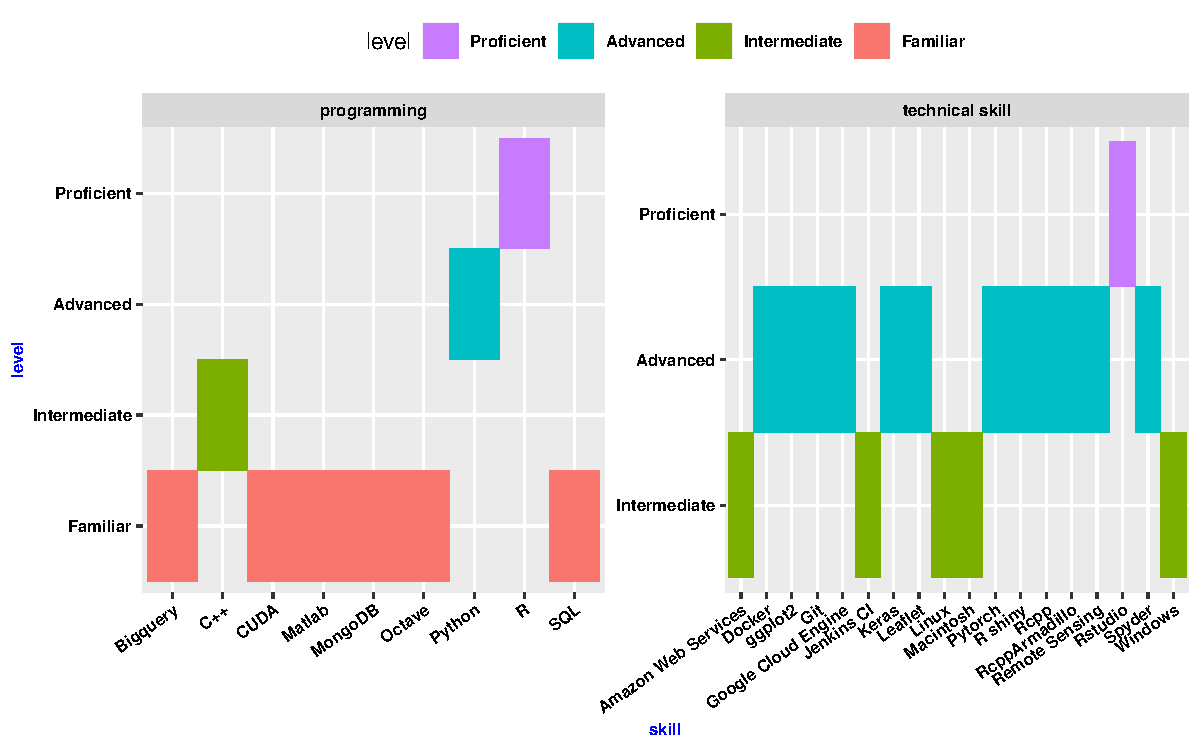
\includegraphics[width=7.6in,height=4.5in]{cv_files/figure-latex/unnamed-chunk-6-1} \end{flushleft}

\hypertarget{geospatial-analysis-timeline}{%
\section{Geospatial Analysis
(Timeline)}\label{geospatial-analysis-timeline}}

\begin{flushleft}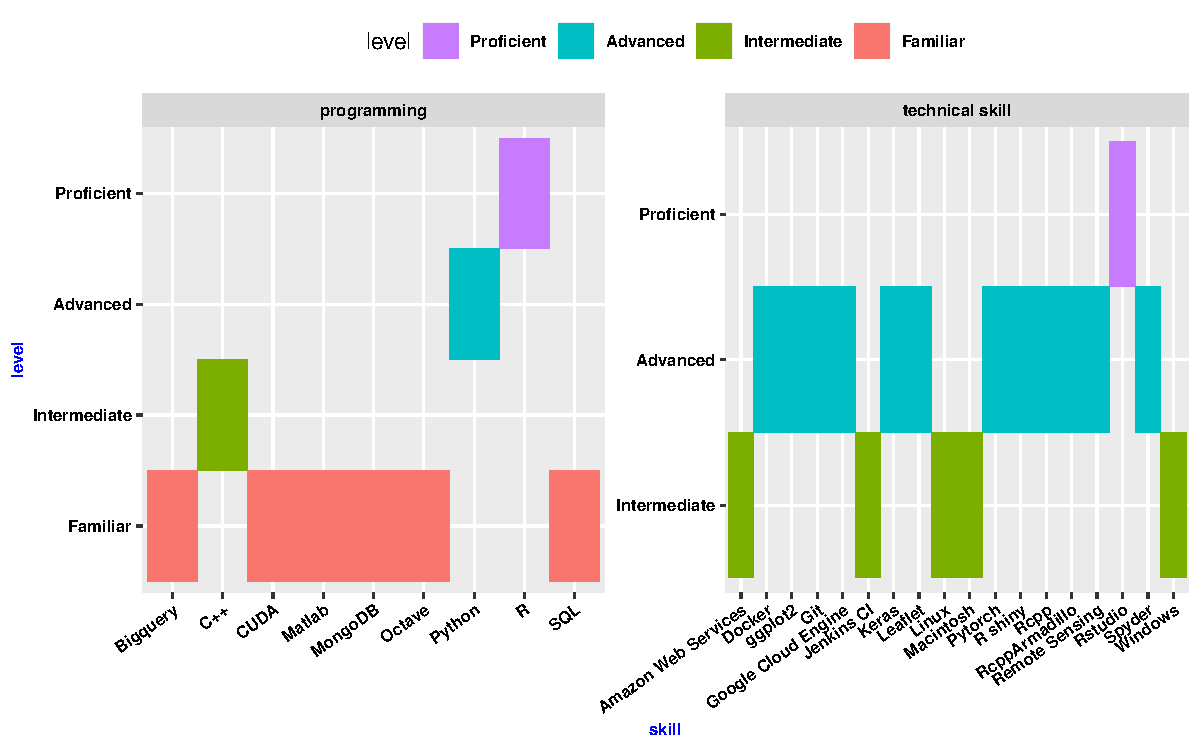
\includegraphics[width=7.6in,height=4.5in]{cv_files/figure-latex/unnamed-chunk-7-1} \end{flushleft}

\pagebreak

\bigskip
\bigskip

\hypertarget{personal-data}{%
\section{Personal Data}\label{personal-data}}

\bigskip

\begin{table}[H]
\centering\begingroup\fontsize{9}{11}\selectfont

\begin{tabular}{>{}l>{\raggedright\arraybackslash}p{30em}}
\toprule
\textcolor{blue}{\textbf{Date of Birth}} & 06th  September 1976\\
\textcolor{blue}{\textbf{Sex}} & Male\\
\textcolor{blue}{\textbf{Mother’s Name}} & Parthena Totska\\
\textcolor{blue}{\textbf{Place of Birth}} & Greece\\
\textcolor{blue}{\textbf{Martial Status}} & Single\\
\addlinespace
\textcolor{blue}{\textbf{Health}} & Irritable Bowel Syndrome (IBS).  IBS affects about 1 out of 10 people according to the International Foundation for functional gastrointestinal disorders (IFFGD)\\
\textcolor{blue}{\textbf{Driving License}} & Car,  Motorcycle\\
\textcolor{blue}{\textbf{triathlon}} & from 2007 to 2010 I was an amateur triathlete\\
\textcolor{blue}{\textbf{trail running}} & Since 2006 I participate occasionally in trail running competitions\\
\textcolor{blue}{\textbf{Free time Activities}} & running, swimming, cycling, tennis playing, watching movies\\
\bottomrule
\end{tabular}
\endgroup{}
\end{table}

\bigskip
\bigskip

\hypertarget{publications}{%
\section{Publications}\label{publications}}

\begin{cventries}
    \cventry{fastText: Efficient learning of word representations and sentence classification using R (R Package Version 1.0. 2)}{L Mouselimis}{}{2022}{}\vspace{-4.0mm}
    \cventry{KernelKnn: kernel k nearest Neighbors}{L Mouselimis}{URL: https://CRAN. R-project. org/package= KernelKnn}{2021}{}\vspace{-4.0mm}
    \cventry{ClusterR: Gaussian mixture models, k-means, mini-batch-kmeans, k-medoids and affinity propagation clustering}{L Mouselimis, C Sanderson, R Curtin, S Agrawal, B Frey, D Dueck}{R package version}{2019}{}\vspace{-4.0mm}
    \cventry{elmNNRcpp: The extreme learning machine algorithm}{L Mouselimis, A Gosso}{R package}{2018}{}\vspace{-4.0mm}
    \cventry{OpenImageR: an image processing Toolkit}{L Mouselimis}{R package version}{2017}{}\vspace{-4.0mm}
\end{cventries}

\end{document}
